\documentclass[../poliXuniversity_hospital_(USP)_report.tex]{subfiles}

\begin{document}

\chapter{Versão 3 robô hospitalar}

\section{Carenagem}
Em busca de um design mais estético e um formato geométrico mais favorável a segurança foi desenvolvido uma nova carenagem de plastico PLA para o robo. A carenagem recebeu as cores do HU e foi contemplada com diversas motificações técnicas. Foi reduzido o número de sensores e reposicionado em função da simplificação do projeto e otimização do sensoriamento, o lidar foi reposicionado para parte inferior garantindo uma movimentação mais segura. Uma tela de para interface com ususario foi adicionada juntamente com um sistema de sons e iluminação led interna e inferior.

\begin{figure}[h]
\centering

    \caption{Hema Bot}
    \begin{minipage}{0.5\textwidth}
        \centering
        \centering % para centralizarmos a figura
        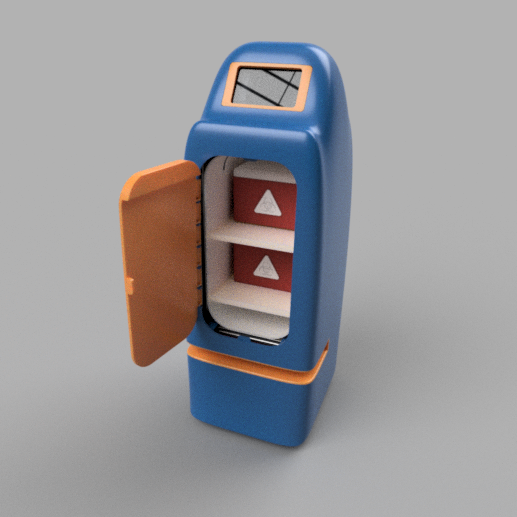
\includegraphics[width=7cm]{images/V3_aberta_angulada.png}
    \end{minipage}\hfill
    \begin{minipage}{0.5\textwidth}
        \centering
        \centering % para centralizarmos a figura
        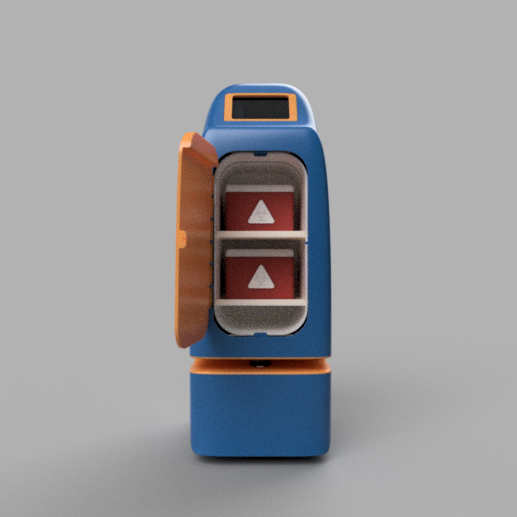
\includegraphics[width=7cm]{images/V3_aberta_frontal.png}

    \end{minipage}\hfill
    \caption*{Fonte: Autor}
    \label{figura: Sistema Golgi}
        
\end{figure}

\section{Modulos embarcados}
Se adaptando as mudanças na carenagem juntamente com a tentativa de simplificar o projeto em termos de intercomunicação entre microcontroladores e organização do hardware(cabos e módulos) no interioro do robo, todos os 5 módulos utilizados anteriormente foram reduzidos a um só.

\begin{figure}[h]
\centering

    \begin{minipage}{0.5\textwidth}
        \centering
        
        \caption{Modulo Hema Bot}
        \centering % para centralizarmos a figura
        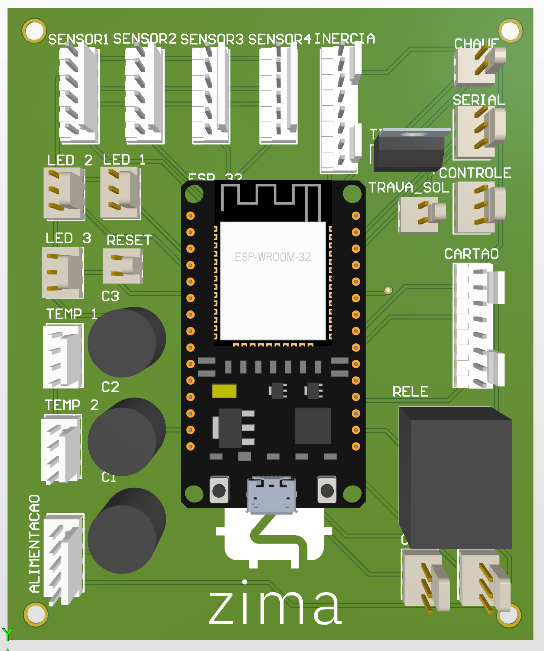
\includegraphics[width=7cm]{images/placa_hema.png}
        \label{figura: Módulo Hmea Bot}
    \end{minipage}\hfill
    \begin{minipage}{0.5\textwidth}
        \centering
        \caption{Esquemático módulo Hema Bot}
        \centering % para centralizarmos a figura
        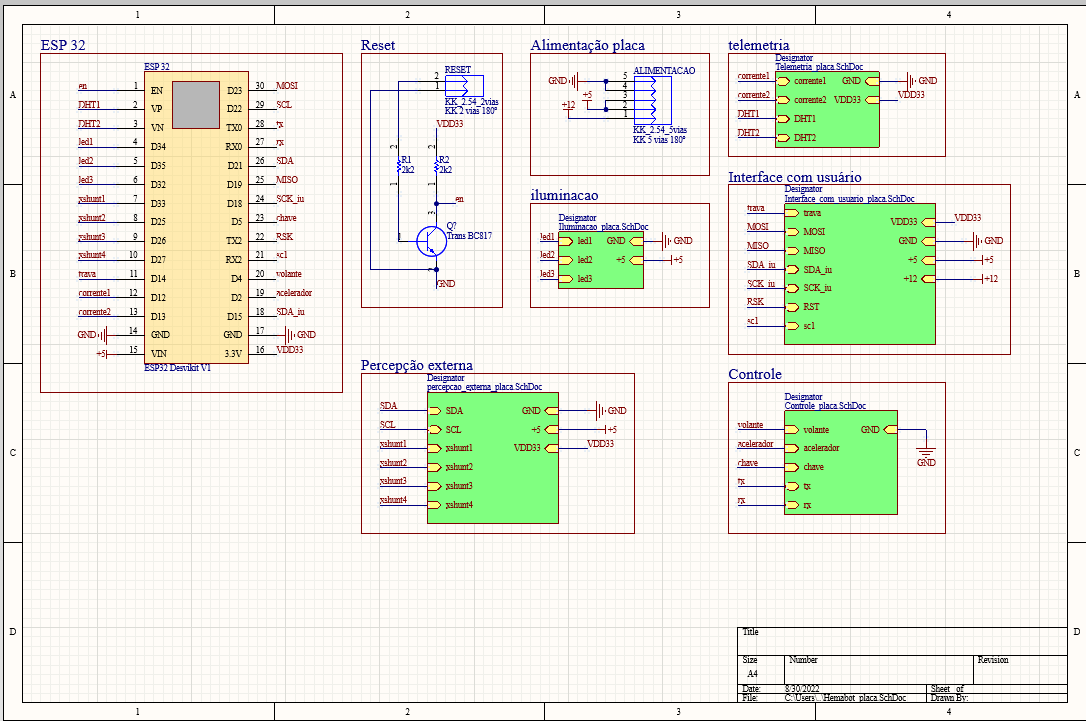
\includegraphics[width=7cm]{images/esquematico_hema.png}
        \label{figura: Esquemático modulo Hema Bot}

    \end{minipage}\hfill
    \caption*{Fonte: Autor}
        
\end{figure}

\end{document}